% <-- chapter -->
\chapter{Configurazione del server}
\label{ch:server}


% <-- section -->
\section{Overview della configurazione e prerequisiti}
\label{sec:overview_server}

In questo capitolo andremo a installare e configurare \it{OpenVPN server} sulla VPS di OVHCloud.

Per facilitare la configurazione e il testing, supponiamo di partire da una topologia che contiene solo il server openvpn e un generico client. Come da specifiche il Server deve avere a disposizione un'ip pubblico e il client deve essere il più generico possibile, lo supponiamo quindi sotto a un NAT.

Supponiamo inoltre che l'ip pubblico del \it{Server} sia \code{51.178.141.119}, si avrà quindi una configurazione iniziale come in figura \ref{fig:diag-simple_ips}.


\newsavebox{\myimage}
\begin{figure}[H]
    \centering%
    \savebox{\myimage}{
        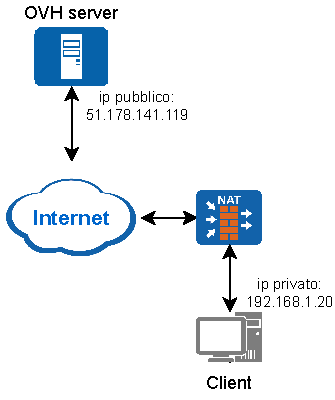
\includegraphics[width=0.45\textwidth]{immagini/diag-simple_ips}
    }
    \begin{subfigure}{0.4\textwidth}
        \centering
        \usebox{\myimage}
        \caption{Configurazione di partenza per questo capitolo.}
        \label{fig:diag-simple_ips}
    \end{subfigure}
    \hfill%
    \begin{subfigure}{0.5\textwidth}
        \centering
        \raisebox{\dimexpr.5\ht\myimage-.5\height\relax}{
            \includegraphics[height=1.15\linewidth]{immagini/diag-simple_ips_vpn}
        }
        \caption{Configurazione virtuale da raggiungere per questo capitolo.}
        \label{fig:diag-simple_ips_vpn}
    \end{subfigure}%
    \caption{Configurazione di partenza e di obbiettivo per questo capitolo. \cite{icons}}
\end{figure}

Per instaurare una comunicazione bidirezionale tra il server e il client, si dovrà configurare opportunamente una rete VPN, che risulterà nella configurazione rappresentata in figura \ref{fig:diag-simple_ips_vpn}.

% TODO maybe cut this
I pacchetti necessari per questo capitolo sono \code{openvpn}, \code{easy-rsa} e un editor di testo, che possono essere installati con:

\begin{bashcode}{Server}{}
$ sudo apt-get update
$ sudo apt-get install -y openvpn easy-rsa vim
\end{bashcode}

% <-- section -->
\section{Creazione della Public key infrastructure}
\label{sec:pki_ca}

Per la gestione dell'autenticazione dei client alla VPN è necessario creare una \it{PKI}, come descritto nella sezione \ref{subsec:auth}, per una maggiore sicurezza è indicato separare la \it{Certificate Authority} dal \it{Server OpenVPN}.

La gestione della PKI viene fatta usando l'utility \it{easy-rsa}, possiamo riassumere i comandi principali della sua creazione nel seguente schema:

\begin{figure}[H]
    \centering
    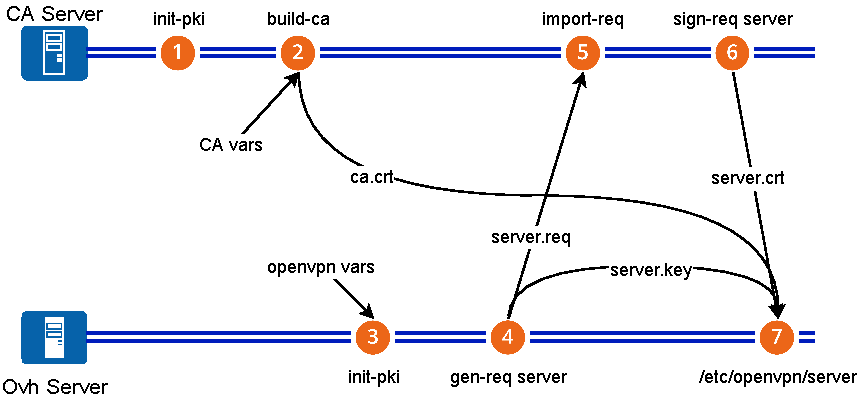
\includegraphics[width=1\linewidth]{immagini/diag-firma_certificato_ca}
    \caption{Diagramma per schematizzare la procedura di creazione della CA.}
    \label{fig:diag-firma_certificato_ca}
\end{figure}

% TODO fare in modo che sotto fa riferimento al diagramma
\subsection{Creazione della CA}

% TODO !
Supponiamo quindi di usare un secondo server chiamato \textit{Server CA}, i suoi requisiti sono: SO Ubuntu e connessione a internet.


Andiamo quindi a crearla, nella home ad esempio (passaggio 1 fig.\ref{fig:diag-firma_certificato_ca}):

\begin{bashcode}{Server CA}{}
$ mkdir ~/openvpn-ca
$ ln -s /usr/share/easy-rsa/* ~/openvpn-ca/
$ chmod 700 /home/ubuntu/openvpn-ca/
$ cd openvpn-ca/
$ ./easyrsa init-pki
init-pki complete; you may now create a CA or requests.
Your newly created PKI dir is: /home/ubuntu/openvpn-ca/pki
$ la
easyrsa  openssl-easyrsa.cnf  pki  vars.example  x509-types
\end{bashcode}

Ora si devono personalizzare le variabili \code{vars}, si può sia partire da un file vuoto oppure modificare \code{vars.example} per poi rinominarlo \code{vars}.
Andiamo quindi a creare un nuovo file vars:

% TODO è of lasciare queste?
\begin{bashcode}{Server CA}{}
$ vim vars
set_var EASYRSA_REQ_COUNTRY  "IT"
set_var EASYRSA_REQ_PROVINCE "MC"
set_var EASYRSA_REQ_CITY     "Recanati"
set_var EASYRSA_REQ_ORG      "Esse-ti"
set_var EASYRSA_REQ_EMAIL    "s.gasparrini@esse-ti.it"
set_var EASYRSA_REQ_OU       "Esse-ti"
set_var EASYRSA_REQ_CN       "openvpn-ca"

set_var EASYRSA_ALGO         "ec"
set_var EASYRSA_DIGEST       "sha512"
\end{bashcode}

Le variabili nel primo blocco determinano i dati che poi verranno registrati nei certificati.

Le ultime 2 sono opzioni di sicurezza, in particolare si setta l'algoritmo di cifratura %TODO add info

A questo punti si deve lanciare il comando \code{build-ca} per costruire la CA (passaggio 2 fig.\ref{fig:diag-firma_certificato_ca}):

\begin{bashcode}{Server CA}{}
$ ./easyrsa build-ca

Note: using Easy-RSA configuration from: ./vars

Using SSL: openssl OpenSSL 1.1.1f  31 Mar 2020

Enter New CA Key Passphrase: 
Re-Enter New CA Key Passphrase: 
read EC key
writing EC key

You are about to be asked to enter information that will be incorporated
into your certificate request.
What you are about to enter is what is called a Distinguished Name or a DN.
There are quite a few fields but you can leave some blank
For some fields there will be a default value,
If you enter '.', the field will be left blank.
-----
Common Name (eg: your user, host, or server name) [Easy-RSA CA]:

CA creation complete and you may now import and sign cert requests.
Your new CA certificate file for publishing is at:
/home/ubuntu/openvpn-ca/pki/ca.crt
    
\end{bashcode}

Eseguendo il comando verrà chiesto di inserire una passshare, che verrà usata per criptare la chiave privata appena generata. Il secondo prompt è relativo al nome da dare alla certificazione, in questo caso è stato lasciato il valore di default \code{Easy-RSA CA}.

% <-- section -->
\subsection{Configurazione della PKI di OpenVPN}
\label{sec:pki_openvpn}

Il procedimento è simile al precedente, ma questa volta va eseguito sul \it{server}.

Creiamo quindi una cartella per ospitare la PKI, es \code{~/openvpn-pki}, e linkiamo \code{easy-rsa}. Inoltre limitiamo i permessi all'utente non root che stimao usando, in questo caso "ubuntu".

\begin{bashcode}{Server}{}
$ mkdir ~/openvpn-pki
$ ln -s /usr/share/easy-rsa/* ~/openvpn-pki/
$ sudo chown ubuntu ~/openvpn-pki/
$ chmod 700 ~/openvpn-pki/
$ cd ~/openvpn-pki/
\end{bashcode}

Andiamo a creare un file \code{vars}:

\begin{bashcode}{Server}{}
$ vim vars
set_var EASYRSA_ALGO    "ec"
set_var EASYRSA_DIGEST  "sha512"
\end{bashcode}
 
Concludiamo la creazione della PKI con il comando:

\begin{bashcode}{Server}{}
$ ./easyrsa init-pki
Note: using Easy-RSA configuration from: ./vars

init-pki complete; you may now create a CA or requests.
Your newly created PKI dir is: /home/ubuntu/openvpn-pki/pki
\end{bashcode}

\subsection{Creazione della chiave privata del server OpenVPN}

A questo punto il server OpenVPN ha tutti i prerequisiti per creare una sua chiave privata e relativa \it{Certificate Signing Request}. 

Come nome è stato scelto "server":

\begin{bashcode}{Server}{}
$ ./easyrsa gen-req server nopass

Note: using Easy-RSA configuration from: ./vars

Using SSL: openssl OpenSSL 1.1.1f  31 Mar 2020
Generating an EC private key
writing new private key to '/home/ubuntu/openvpn-pki/pki/private/server.key.438W2xM0g9'
-----
You are about to be asked to enter information that will be incorporated
into your certificate request.
What you are about to enter is what is called a Distinguished Name or a DN.
There are quite a few fields but you can leave some blank
For some fields there will be a default value,
If you enter '.', the field will be left blank.
-----
Common Name (eg: your user, host, or server name) [server]:

Keypair and certificate request completed. Your files are:
req: /home/ubuntu/openvpn-pki/pki/reqs/server.req
key: /home/ubuntu/openvpn-pki/pki/private/server.key
\end{bashcode}

La chiave \code{server.key} va copiata nell'apposita cartella.

\begin{bashcode}{Server}{}
$ sudo cp /home/ubuntu/openvpn-pki/pki/private/server.key /etc/openvpn/server/
\end{bashcode}

Il secondo file creato, \code{server.req}, corrisponde a una \textit{Certificate Signing Request (CSR)} che va firmata e validata dalla CA. 

% TODO da togliere
In questo modo ogni client che si fida della CA si fiderà di conseguenza del server OpenVPN 


\subsection{Firma del certificato OpenVPN dalla CA}
\label{sec:sign_openvpn}

Dobbiamo quindi copiare il file \code{server.req} nel \textit{server CA}, possiamo qualunque metodo purchè sia sicuro, ad esempio con \code{scp}:

\begin{bashcode}{Server CA}{}
$ scp ubuntu@openvpn_server:/home/ubuntu/openvpn-pki/pki/reqs/server.req /tmp
\end{bashcode}

Dobbiamo quindi spostarci sul server CA e importare la \textit{certificate request} e firmarlo:

\begin{bashcode}{Server CA}{}
$ cd ~/openvpn-ca
$ ./easyrsa import-req /tmp/server.req server
$ ./easyrsa sign-req server server
Using configuration from /home/ubuntu/openvpn-ca/pki/safessl-easyrsa.cnf
Check that the request matches the signature
Signature ok
The Subject\'s Distinguished Name is as follows
commonName            :ASN.1 12:'server'
Certificate is to be certified until Mar 11 15:50:45 2025 GMT (1080 days)

Write out database with 1 new entries
Data Base Updated
\end{bashcode}

Verrà creato un file in \code{~/openvpn-ca/pki/issued} chiamato \code{server.crt} che conterrà la chiave pubblica che verrà usata dal server openvpn e inoltre la firma della CA.

Ora si devono copiare i file \code{ca.crt} e \code{server.crt} dal \textit{server CA} al \textit{server OpnenVPN}:

% TODO unire il codice

\begin{bashcode}{Server}{}
$ scp ubuntu@ca_server:/home/ubuntu/openvpn-ca/pki/issued/server.crt /tmp
$ scp ubuntu@ca_server:/home/ubuntu/openvpn-ca/pki/ca.crt /tmp
\end{bashcode}

Possiamo quindi tornare sul \textit{server OpenVPN} e copiare i 2 file da \code{/tmp} a \\\code{/etc/openvpn/server}:

\begin{bashcode}{Server}{}
$ sudo cp /tmp/server.crt /etc/openvpn/server
$ sudo cp /tmp/ca.crt /etc/openvpn/server
\end{bashcode}


% <-- section -->
\section{Generazione della \textit{tls-crypt pre-shared key}}
\label{sec:tls-crypt}

Per aumentare ulteriormente la sicurezza del nostro \textit{server OpenVPN} possiamo creare un'ulteriore chiave, che consiste un una chiave \it{preshared} che verrà inserita in tutte le configurazioni e serve a offuscare il certificato in fase di validazione. Quindi in caso di attacco si dovrà conoscere anche questa chiave.

% TODO merge i 2 pezzi di codice
La creazione va fatta sul \it{server OpenVPN}:

\begin{bashcode}{Server}{}
$ cd ~/openvpn-pki/
$ openvpn --genkey --secret ta.key
\end{bashcode}

il file generato \code{ta.key} dovrà essere copiato nella directory del server openvpn:

\begin{bashcode}{Server}{}
$ sudo cp ta.key /etc/openvpn/server
\end{bashcode}


% <-- section -->
\section{Generazione delle chiavi per i clients}
\label{sec:client_keys}

\begin{figure}[H]
    \centering
    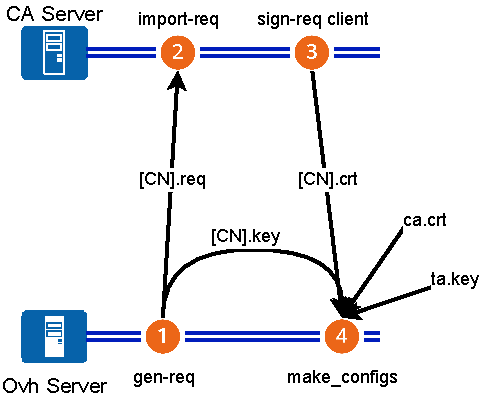
\includegraphics[width=0.6\linewidth]{immagini/diag-firma_certificato_client}
    \caption{Diagramma per schematizzare la procedura di firma di un certificato client. \cite{icons}}
    \label{fig:diag-firma_certificato_client}
\end{figure}

% TODO fare in modo che il testo sotto faccia riferimento al diagramma

Creiamo una cartella nella \it{home} che ospiterà le chiavi dei \it{client} e le configurazioni openvpn:

\begin{bashcode}{Server}{}
$ mkdir -p ~/client-configs/keys
$ chmod -R 700 ~/client-configs
\end{bashcode}

Creiamo quindi un certificato per un \it{client}:

\begin{bashcode}{Server}{}
$ cd ~/openvpn-pki/
$ ./easyrsa gen-req client1 nopass
\end{bashcode}

Ora dobbiamo copiare \code{client1.key} nella directory appena creata, e \code{client1.req} va copiato nel server CA per essere firmato:

\begin{bashcode}{Server}{}
$ cp pki/private/client1.key ~/client-configs/keys/
$ scp /home/ubuntu/openvpn-pki/pki/reqs/client1.req ubuntu@ca_server:/tmp
\end{bashcode}

Dobbiamo quindi spostarci sul server CA e importare la \textit{certificate request} e firmarla:

\begin{bashcode}{Server CA}{}
$ cd ~/openvpn-ca
$ ./easyrsa import-req /tmp/client1.req client1
$ ./easyrsa sign-req client client1
Using configuration from /home/ubuntu/openvpn-ca/pki/safessl-easyrsa.cnf
Check that the request matches the signature
Signature ok
The Subject\'s Distinguished Name is as follows
commonName            :ASN.1 12:'client1'
Certificate is to be certified until Mar 16 13:15:09 2025 GMT (1080 days)

Write out database with 1 new entries
Data Base Updated
\end{bashcode}

Per poi ricopiare dal server CA al server openvpn il certificato firmato:

% TODO unire il codice

\begin{bashcode}{Server}{}
$ scp ubuntu@ca_server:/home/ubuntu/openvpn-ca/pki/issued/client1.crt /tmp
\end{bashcode}

Quindi ci dobbiamo spostare sul server OpenVPN e copiare le chiavi nella cartella \\\code{client-configs/keys}, in modo da prepararla per la creazione delle configurazioni OpenVPN. È necessario inoltre cambiare i permessi dei file rendendoli accessibili all'utente Ubuntu:

\begin{bashcode}{Server}{}
$ cp /tmp/client1.crt ~/client-configs/keys/
$ cp ~/openvpn-pki/ta.key ~/client-configs/keys/
$ sudo cp /etc/openvpn/server/ca.crt ~/client-configs/keys/
$ sudo chown ubuntu:ubuntu ~/client-configs/keys/*
\end{bashcode}


% <-- section -->
\section{Creazione del file di configurazione del server OpenVPN}
\label{sec:server_config}

Il server openvpn viene configurato attraverso \code{/etc/openvpn/server/server.conf}, per non partire da una configurazione vuota si può usare la configurazione di esempio offerta da openvpn:

\begin{bashcode}{Server}{}
$ cd /etc/openvpn/server/
$ sudo wget "https://raw.githubusercontent.com/OpenVPN/openvpn/\
                master/sample/sample-config-files/server.conf"
\end{bashcode}

Dobbiamo quindi modificare il file e cambiare alcune configurazioni, per facilitare la lettura sarà incluso il numero riga modificato:

% TODO da controllare se sono tutte le modifiche
\begin{bashcode}{Server}{}
$ sudo vim server.conf
85  dh none             # non sonos stati usati i parametri Diffie-Hellman
92  topology subnet     # topologia raccomandata
244 ;tls-auth ta.key 0 # This file is secret
245 tls-crypt ta.key    # selezione della preshared key
253 cipher AES-256-GCM  # selezione della cifratura scelta
275 user nobody         # utente che eseguirà il server openvpn, in modo da 
                        #  restringere i permessi
276 group nogroup       # stassa cosa per il gruppo
318 auth sha256         # selezione del metodo di autenticazione
\end{bashcode}


% <-- section -->
\section{Configurazioni sulla network stack del server openvpn}
\label{sec:network_stack}

Per abilitare l'\textit{ip forwarding} si dovrà modificare il file \code{/etc/sysctl.conf}, il comando successivo serve a ricaricare le configurazioni dai file:

\begin{bashcode}{Server}{}
$ sudo vim /etc/sysctl.conf
69 net.ipv4.ip_forward = 1
$ sudo sysctl -p
net.ipv4.ip_forward = 1
\end{bashcode}


% <-- section -->
\section{Configurazione del firewall}
\label{sec:firewall}

Sulla VPS scelta è presente il firewall \code{firewalld}, ma per una più semplice configurazione è consigliato di disattivarlo e installare \code{ufw}:

\begin{bashcode}{Server}{}
$ sudo systemctl mask firewalld
$ sudo systemctl stop firewalld
$ sudo apt-get install ufw
$ sudo ufw allow ssh
Rule added
Rule added (v6)
$ sudo ufw enable
\end{bashcode}

È importantissimo ricordarsi di consentire l'SSH prima di abilitare il firewall, altrimenti si perderà l'accesso alla VPS.


\subsection{Configurazione del NAT}

Per far si che i pacchetti provenienti dalla \it{VPN} entrino nella network stack del \it{server} si deve aggiungere una regola di \it{NAT} nel firewall. Per farlo si deve conoscere quale è l'interfaccia di rete del \it{server}, cioè quella che ha come ip il suo ip pubblico:

\begin{bashcode}{Server}{}
$ ip addr
[...]
2: ens3: <BROADCAST,MULTICAST,UP,LOWER_UP> mtu 1500 qdisc mq state UP group default qlen 1000
    link/ether a6:23:5f:48:ba:de brd ff:ff:ff:ff:ff:ff
    inet 51.178.141.119/20 brd 51.178.141.255 scope global dynamic ens3
       valid_lft 1857sec preferred_lft 1857sec
    inet6 fe80::23:bfff:ac24:aace/64 scope link
       valid_lft forever preferred_lft forever
[...]
\end{bashcode}

In questo caso il nome dell'interfaccia di rete è \it{ens3}, possiamo quindi procedere con la configurazione del firewall, si andrà a modificare il file \code{/etc/ufw/before.rules} e aggiungere la regola di NAT:

\begin{bashcode}{Server}{}
$ sudo vim /etc/ufw/before.rules
# ## rules.before
# ## Rules that should be run before the ufw command line added rules. Custom
# rules should be added to one of these chains:
# ufw-before-input
# ufw-before-output
# ufw-before-forward
#

# START OPENVPN RULES
# NAT table rules
*nat
:POSTROUTING ACCEPT [0:0]
# Allow traffic from OpenVPN client to ens3 
-A POSTROUTING -s 10.8.0.0/24 -o ens3 -j MASQUERADE
COMMIT
# END OPENVPN RULES


# Don't delete these required lines, otherwise there will be errors
*filter
. . .
\end{bashcode}

Nella modifica del file si deve stare attenti a inserire la nuova regola in cima al file e sotto i commenti iniziali, è inoltre importante inserire i commenti nella regola.

\subsection{Configurazione del packet forwarding}

Precedentemente abbiamo abilitato il forwarding nella network stack del server, ora si deve abilitare la corrispondente opzione nel firewall. Si deve quindi cambiare la regola di default per i pacchetti inoltrati da \code{DROP} ad \code{ACCEPT}.

Per farlo si deve modificare il file \code{/etc/default/ufw}:

\begin{bashcode}{Server}{}
$ sudo vim /etc/default/ufw
DEFAULT_FORWARD_POLICY="ACCEPT"
\end{bashcode}

\subsection{Conclusione della configurazione del firewall}

Per concludere la configurazione si deve abilitare la porta relativa alla vpn, in questo caso \code{1194}, e riavviare il firewall:

\begin{bashcode}{Server}{}
$ sudo ufw allow 1194/udp
$ sudo ufw reload
$ sudo ufw status
Status: active
To              Action      From
--              ------      ----
22              ALLOW       Anywhere
1194/udp        ALLOW       Anywhere
22 (v6)         ALLOW       Anywhere (v6)
1194/udp (v6)   ALLOW       Anywhere (v6)
\end{bashcode}


% <-- section -->
\section{Avvio del server OpenVPN}
\label{sec:start_server}

Ora che la configurazione del server è in una situazione stabile possiamo avviarlo:

\begin{bashcode}{Server}{}
$ sudo systemctl enable openvpn-server@server.service
$ sudo systemctl start openvpn-server@server.service
$ sudo systemctl status openvpn-server@server.service
● openvpn-server@server.service - OpenVPN service for server
     Loaded: loaded (/usr/lib/systemd/system/openvpn-server@.service; enabled; vendor preset: disabled)
     Active: active (running) since Mon 2022-04-18 13:08:44 CEST; 4h 22min ago
       Docs: man:openvpn(8)
             https://community.openvpn.net/openvpn/wiki/Openvpn24ManPage
             https://community.openvpn.net/openvpn/wiki/HOWTO
   Main PID: 436 (openvpn)
     Status: "Initialization Sequence Completed"
      Tasks: 1 (limit: 9488)
     Memory: 4.8M
        CPU: 199ms
     CGroup: /system.slice/system-openvpn\x2dserver.slice/openvpn-server@server.service
             └─436 /usr/bin/openvpn --status /run/openvpn-server/status-server.log --status-version 2 --suppress-timestamps --config server.conf

Apr 18 13:08:44 server openvpn[436]: TUN/TAP device tun0 opened
Apr 18 13:08:44 server openvpn[436]: Incoming Control Channel Encryption: Cipher 'AES-256-CTR' initialized with 256 bit key
Apr 18 13:08:44 server openvpn[436]: Incoming Control Channel Encryption: Using 256 bit message hash 'SHA256' for HMAC authentication
Apr 18 13:08:44 server openvpn[436]: net_addr_v4_add: 10.8.0.1/24 dev tun0
Apr 18 13:08:44 server openvpn[436]: UDPv4 link local (bound): [AF_INET][undef]:1194
Apr 18 13:08:44 server openvpn[436]: UDPv4 link remote: [AF_UNSPEC]
Apr 18 13:08:44 server openvpn[436]: MULTI: multi_init called, r=256 v=256
Apr 18 13:08:44 server openvpn[436]: IFCONFIG POOL IPv4: base=10.8.0.2 size=253
Apr 18 13:08:44 server openvpn[436]: IFCONFIG POOL LIST
Apr 18 13:08:44 server openvpn[436]: Initialization Sequence Completed
\end{bashcode}
 
Il comando \code{systemctl enable} abilita il servizio per essere avviato all'avvio della macchina, mentre \code{systemctl start} lo avvia immediatamente. Con il comando \code{systemctl status} si può verificare lo stato del servizio, si vede che il servizio è \it{active (running)}.

% <-- section -->
\section{Script per la creazione delle configurazioni dei client}
\label{sec:script_client}

Per facilitare la creazione dei file di configurazione dei client, \code{clientX.ovpn}, andremo a creare un apposito script bash. Per prima cosa si deve scaricare e personalizzare la configurazione base del client:

\begin{bashcode}{Server}{}
$ cd ~/client-configs/
$ wget "https://raw.githubusercontent.com/OpenVPN/openvpn\
            /master/sample/sample-config-files/client.conf" \
                -O base.conf
$ vim base.conf
42   remote 51.178.141.119 1194     # va messo l'ip e la porta del server OpenVPN
88   ;ca ca.crt                     # non useremo i file esterni ma ingloberemo 
89   ;cert client.crt               #   questi file in un file direttamente nella
90   ;key client.key                #   configurazione del client
108  ;tls-auth ta.key 1             # 
116  cipher AES-256-GCM             # cifratura usata
117  auth SHA256                    # autenticazione usata
118  key-direction 1                # indica che è un client
\end{bashcode}

Ora creiamo lo script bash \code{make\_config.sh}:

\begin{bashcode}{Server}{}
$ vim make_config.sh
#!/bin/bash

# usage:
# \$ make\_config.sh client1
# will use [ca.crt, client1.crt, client1.key, ta.key] to create client1.ovpn
    
KEY_DIR=~/client-configs/keys
OUTPUT_DIR=~/client-configs/files
BASE_CONFIG=~/client-configs/base.conf
    
cat ${BASE_CONFIG} \
    <(echo -e '<ca>') \
    ${KEY_DIR}/ca.crt \
    <(echo -e '</ca>\n<cert>') \
    ${KEY_DIR}/${1}.crt \
    <(echo -e '</cert>\n<key>') \
    ${KEY_DIR}/${1}.key \
    <(echo -e '</key>\n<tls-crypt>') \
    ${KEY_DIR}/ta.key \
    <(echo -e '</tls-crypt>') \
    > ${OUTPUT_DIR}/${1}.ovpn
$ chmod 700 make_config.sh
\end{bashcode}

% TODO da riscrivere!
Lo scopo di questo script è di aggiungere al file \code{base.conf} il certificato della CA, \code{ca.crt}, il certificato e chiave relativi al client per cui si sta creando la configurazione, passato come argomento allo script, e la \it{preshared key}. 

Il tutto viene scritto in un file che ha lo stesso nome del \it{client} per cui si sta creando la configurazione ma \code{.ovpn}.

Quindi per creare la configurazione di \it{client 1}:

\begin{bashcode}{Server}{}
$ ./make_config.sh client1
\end{bashcode}

Nella cartella \code{client-configs/files/} si troverà il file di configurazione per il client \\\code{client1.ovpn}.

\section{Test della configurazione}
\label{sec:test_config_server}

Ora che abbiamo un file di configurazione per il client, possiamo testare che la configurazione fino a questo punto sia corretta. 
Per farlo ci spostiamo su una macchina client, con SO Linux ad esempio, e si può connettere il \it{client} alla vpn con la configurazione creata al passo precedente:

\begin{bashcode}{Client}{}
$ sudo openvpn --config client1.ovpn
[...]
Thu Apr 21 12:53:04 2022 Outgoing Data Channel: Cipher 'AES-256-GCM' initialized with 256 bit key
Thu Apr 21 12:53:04 2022 Incoming Data Channel: Cipher 'AES-256-GCM' initialized with 256 bit key
Thu Apr 21 12:53:04 2022 ROUTE_GATEWAY 192.168.1.20/255.255.255.0 IFACE=eth0 HWADDR=02:42:0a:00:04:03
Thu Apr 21 12:53:04 2022 /sbin/ip route add 10.8.0.1/32 via 10.8.0.2
Thu Apr 21 12:53:04 2022 WARNING: this configuration may cache passwords in memory -- use the auth-nocache option to prevent this
Thu Apr 21 12:53:04 2022 Initialization Sequence Completed
\end{bashcode}

Se la configurazione fino a questo punto è corretta si avrà il messaggio \\\code{Initialization Sequence Completed}.

Nel \it{client} si avrà una nuova interfaccia di rete chiamata \code{tun0}, questa è l'interfaccia virtuale creata dalla vpn.

\begin{bashcode}{Client}{}
$ ip addr
2: tun0: <MULTICAST,NOARP,UP,LOWER_UP> mtu 1500 qdisc fq_codel state UNKNOWN group default qlen 500
    link/none 
    inet 10.8.0.2/24 scope global tun0
       valid_lft forever preferred_lft forever
\end{bashcode}

Si può vedere come l'ip assegnato al \it{client} dalla vpn è \code{10.8.0.2}.

Per testare che la connessione sia instaurata correttamente si può usare la utility \code{ping}, ad esempio possiamo fare il ping dal \it{client} verso l'ip interno alla vpn del \it{server}:

\begin{bashcode}{Client}{}
$ ping -c2 10.8.0.1
PING 10.8.0.1 (10.8.0.1) 56(84) bytes of data.
64 bytes from 10.8.0.1: icmp_seq=1 ttl=64 time=0.250 ms
64 bytes from 10.8.0.1: icmp_seq=2 ttl=64 time=0.220 ms
\end{bashcode}

Se nel frattempo si esegue la utility \code{tpcdump} sul server si potranno vedere i pacchetti \it{echo request} ed \it{echo reply}:

\begin{bashcode}{Server}{}
$ sudo tcpdump
listening on tun0, link-type RAW (Raw IP), capture size 262144 bytes
13:11:12.018615 IP 10.8.0.2 > 10.8.0.1: ICMP echo request, id 11, seq 1, length 64
13:11:12.018640 IP 10.8.0.1 > 10.8.0.2: ICMP echo reply, id 11, seq 1, length 64
13:11:13.039993 IP 10.8.0.2 > 10.8.0.1: ICMP echo request, id 11, seq 2, length 64
13:11:13.040018 IP 10.8.0.1 > 10.8.0.2: ICMP echo reply, id 11, seq 2, length 64
\end{bashcode}

Si vede quindi che è possibile una comunicazione bidirezionale tra \it{client}, \code{10.8.0.2}, e \it{server}, \code{10.8.0.1}.